%last updated in April 2002 by Antje Endemann

\documentclass[runningheads]{llncs}
%In order to omit page numbers and running heads
%please use the following line instead of the first command line:
%\documentclass{llncs}.
%Furthermore change the line \pagestyle{headings} to
%\pagestyle{empty}.
\usepackage{graphicx}
\usepackage{url}
\usepackage{color}
\usepackage{amsmath}
\newcommand{\argmin}{\operatornamewithlimits{argmin}}
\newcommand {\afbnote} [1] {{\bf \textcolor{red}{(#1)}}}
\newcommand {\ericnote} [1] {{\bf \textcolor{magenta}{(#1)}}}
\newcommand {\PnP} {P$n$P}
\newcommand {\EPnP} {EP$n$P}
\input{psfig.sty}

\begin{document}

\pagestyle{headings}
%In order to omit page numbers and running heads
%please change this line to
%\pagestyle{empty}
%and change the first command line too, see above.

\mainmatter

\title{Camera pose from face images}

\titlerunning{Camera pose from face images}

\maketitle

\begin{abstract}
We present a method for estimating the distance between a camera and a human head in 2D images from a calibrated camera.  The distance is estimated by solving for the camera pose using Effective Perspective $n$ Point (EP$n$P).  Leading head pose estimation algorithms focus mainly on head orientation (yaw, pitch, and roll) and translations perpendicular to the camera principal axis.  Our contribution is a system that can estimate head pose under large translations parallel to the camera's principal axis.  Our method uses a set of exemplar 3D human heads to estimate the distance between a camera and a previously unseen head.  We present promising experimental results using the Texas 3D Face Recognition Database.
\end{abstract}

\section{Introduction}
When photographing a human head, the subject's appearance can vary dramatically depending on the camera's distance from the subject.
This variation is caused by perspective distortion, and for 3D objects cannot be undone by simply adjusting focal length; see Figure \ref{fig:fiducial_migration} for an illustration using a synthetic head\footnote{Generated using FaceGen (\url{http://www.facegen.com}).}.

This distortion presents a problem for automatic cross-condition face recognition, e.g. webcam-based recognition from social media images.
Even humans find such recognition difficult \cite{liu2003face,liu2006face}.
It is also a source of information, allowing camera pose estimation in cases where the subject is known \cite{ohayon2006robust}.
This information could potentially be used to undistort the images and improve recognition results.

In this paper, we show camera distance estimation from 2D images is possible even when the subject is previously unseen.
Our technique replaces the known-subject assumption with knowledge of the general distribution of fiducials across people.
This distribution turns out to be sufficiently tight to allow surprisingly accurate distance estimation using only a small training set.

The paper is organized as follows.
Section \ref{sec:related} covers related work from psychology and computer vision.
Section \ref{sec:method} explains our method.
In Section \ref{sec:experiments}, we validate our method on the Texas 3D Face Recognition Database.
Section \ref{sec:discussion} is the discussion.

\begin{figure}[ht!]
\centering
\begin{tabular}{ccc}
\includegraphics[width=.33\linewidth]{resources/figures/extracted_fiducial_0006.png} &
\includegraphics[width=.33\linewidth]{resources/figures/extracted_fiducial_0008.png} &
\includegraphics[width=.33\linewidth]{resources/figures/extracted_fiducial_0001.png} \\
\includegraphics[width=.33\linewidth]{resources/figures/extracted_fiducial_0002.png} &
\includegraphics[width=.33\linewidth]{resources/figures/extracted_fiducial_0003.png} &
\includegraphics[width=.33\linewidth]{resources/figures/extracted_fiducial_0004.png} \\
\includegraphics[width=.33\linewidth]{resources/figures/extracted_fiducial_0005.png} &
\includegraphics[width=.33\linewidth]{resources/figures/extracted_fiducial_0007.png} &
\includegraphics[width=.33\linewidth]{resources/figures/fiducial_migration.png}
\end{tabular}
\caption{
A synthetic head viewed from different camera distances, illustrating projective distortion.
Camera distance decreases in the first eight images, indexed in row-major order.
Here, the focal length (zoom) is adjusted to keep the figure at a constant size.
Fiducials are shown as red dots.
In the first image, the camera is far away, resulting in near orthographic projection.
In the eighth image (bottom row, middle column) the camera is very close to the human head.  
The last image is the same as the first, but with fiducial markers from all images.
This illustrates the migration of fiducials as a function of camera distance and focal length. 
} 
\label{fig:fiducial_migration}
\end{figure}

\subsection{Related works} \label{sec:related}
There is previous work on head pose estimation from 2D images; see \cite{murphy2009head} for a recent survey.
However, most methods attempt to recover a subset of the yaw, pitch, and roll of the head with respect to the camera.
To our knowledge, these methods do not attempt to estimate the distance between the camera and head; Figure \ref{fig:head_pose} illustrates the difference.
In this section we discuss works most similar to our own.

\begin{figure}[ht]
\centering
\includegraphics[width=1.0\linewidth]{resources/figures/head_pose.png}
\caption{
An illustration of the six degrees of freedom governing head pose relative to a camera.
Prior work has focused on estimation of yaw, pitch, and roll \cite{murphy2009head}.
In this paper, we assume these parameters are known and estimate camera distance from the subject, shown here as distance along the $z$ axis.
}
\label{fig:head_pose}
\end{figure}

In \cite{liu2003face,liu2006face}, Liu et al. study the effect of face recognition by humans when viewing faces at different perspective convergence angles (effectively focal length or field of view). 
The study involved a training phase in which face images were displayed to a human test subject.
In a later recognition phase the subject was shown images of faces and asked to determine whether each face had been previously displayed.
The field of view was changed to see if this had an effect on recognition. 
Their results show that even humans have a hard time recognizing a face when viewed under different levels of perspective distortion.  
This is a motivating factor since if humans have trouble with this task, a computer vision algorithm will likely also have the same troubles.  
Predicting the distance between camera and face is a first step in mitigating the effects of perspective distortion.

A similar psychology based studied is presented in \cite{perona2007new,bryan2012perspective}. 
Here, Perona et al. investigate the effects of perspective distortion as visual cue for social judgement of faces.  
Human subjects were asked to judge an image of a face in terms of trustworthiness, attractiveness, and competence.  
Their results show that for social judgements, pictures taken up close are generally rated lower, while pictures taken far away have higher ratings.

In automatic camera calibration, camera parameters are recovered using prior information about the imaged scene.
In \cite{deutscher2002automatic}, Deutscher et al. recover camera parameters under the assumption the scene satisfies a Manhattan world criterion.
This is similar to our technque, which assumes human fiducial locations are approximately distributed according to an estimated distribution. 
In \cite{lv2006camera}, Lv et al. use a human subject for calibration, but unlike this work requires multiple frames of video.
In \cite{krahnstoever2005bayesian}, Krahnstoever and Mendonca use a full human body for calibration from a single image, where this work uses just the head.

In \cite{ohayon2006robust}, Ohayon and Rivlin present head tracking as a camera pose estimation problem.  
Prior to head tracking, 3D points are acquired from the head.  
During tracking, correspondences between the 3D points and their imaged 2D points are used to estimate head pose by solving the inverse problem, namely camera pose. 
They use the Perspective $n$-Point (\PnP) formulation to solve for the camera extrinsic parameters (rotation $R$ and translation $T$).  
The \PnP~method is also known as the Location Determination Problem and was first coined in \cite{ransac}.  
In effect, the human head is used as a calibration rig.  
In this paper, the authors show that head pose can be accurately estimated and tracked under varying yaw, pitch, and roll and translations about $x$ and $y$ axes. 
However, they assume knowledge of the ground-truth fiducial locations and do not address dramatic changes in camera distance.

\section{Camera pose estimation from face images using \EPnP} \label{sec:method}
Our work is based on \cite{ohayon2006robust}, but we focus primarily on translation along the $z$-axis, which affects the level of induced perspective distortion.  
We present a method for estimating the pose of a previously unseen human head using a dataset of exemplar human heads. 

\textit{Efficient Perspective $n$-Point (\EPnP):} The method uses \EPnP, a fast, non-iterative, solution to the \PnP~problem \cite{lepetit2009epnp}.  
We use code provided by the authors\footnote{\url{http://cvlab.epfl.ch/software/EPnP}}.
As stated earlier, the \PnP~problem is to estimate the pose of a calibrated camera from $n$ 3D-to-2D correspondences.
In particular, \EPnP~enables us to estimate camera pose based on a set of 2D fiducial locations and their corresponding 3D locations.
% The advantage of \EPnP~is that the computational complexity grows linearly with $n$, whereas other state-of-the-art methods are $O(n^5)$ or even $O(n^8)$.  

\textit{Exemplar 3D heads:} Note the geometric configuration of fiducial features varies from face to face, but in general fiducial locations tend to form clusters, as illustrated in Figure \ref{fig:fiducial_clusters}.
This means the fiducial locations of a new person are likely to be similar to those in an exemplar set.
We take advantage of this by using a set of exemplar 3D heads to estimate the camera pose of a novel head.

\textit{The method:} The method is based on simple averaging, leveraging the observation from the previous paragraph.
Suppose we get an image $I$ of a previously unobserved head.
For each exemplar 3D head $E$, the camera pose is estimated via \EPnP~under the assumption the fiducials of $I$ match the fiducials of $E$.
This assumption is incorrect, but as mentioned in the last paragraph, it is not far off.
The estimated camera distance for $I$ is just the average of the camera distances across all the exemplars.

\begin{figure}[h]
\centering
\begin{tabular}{cc}
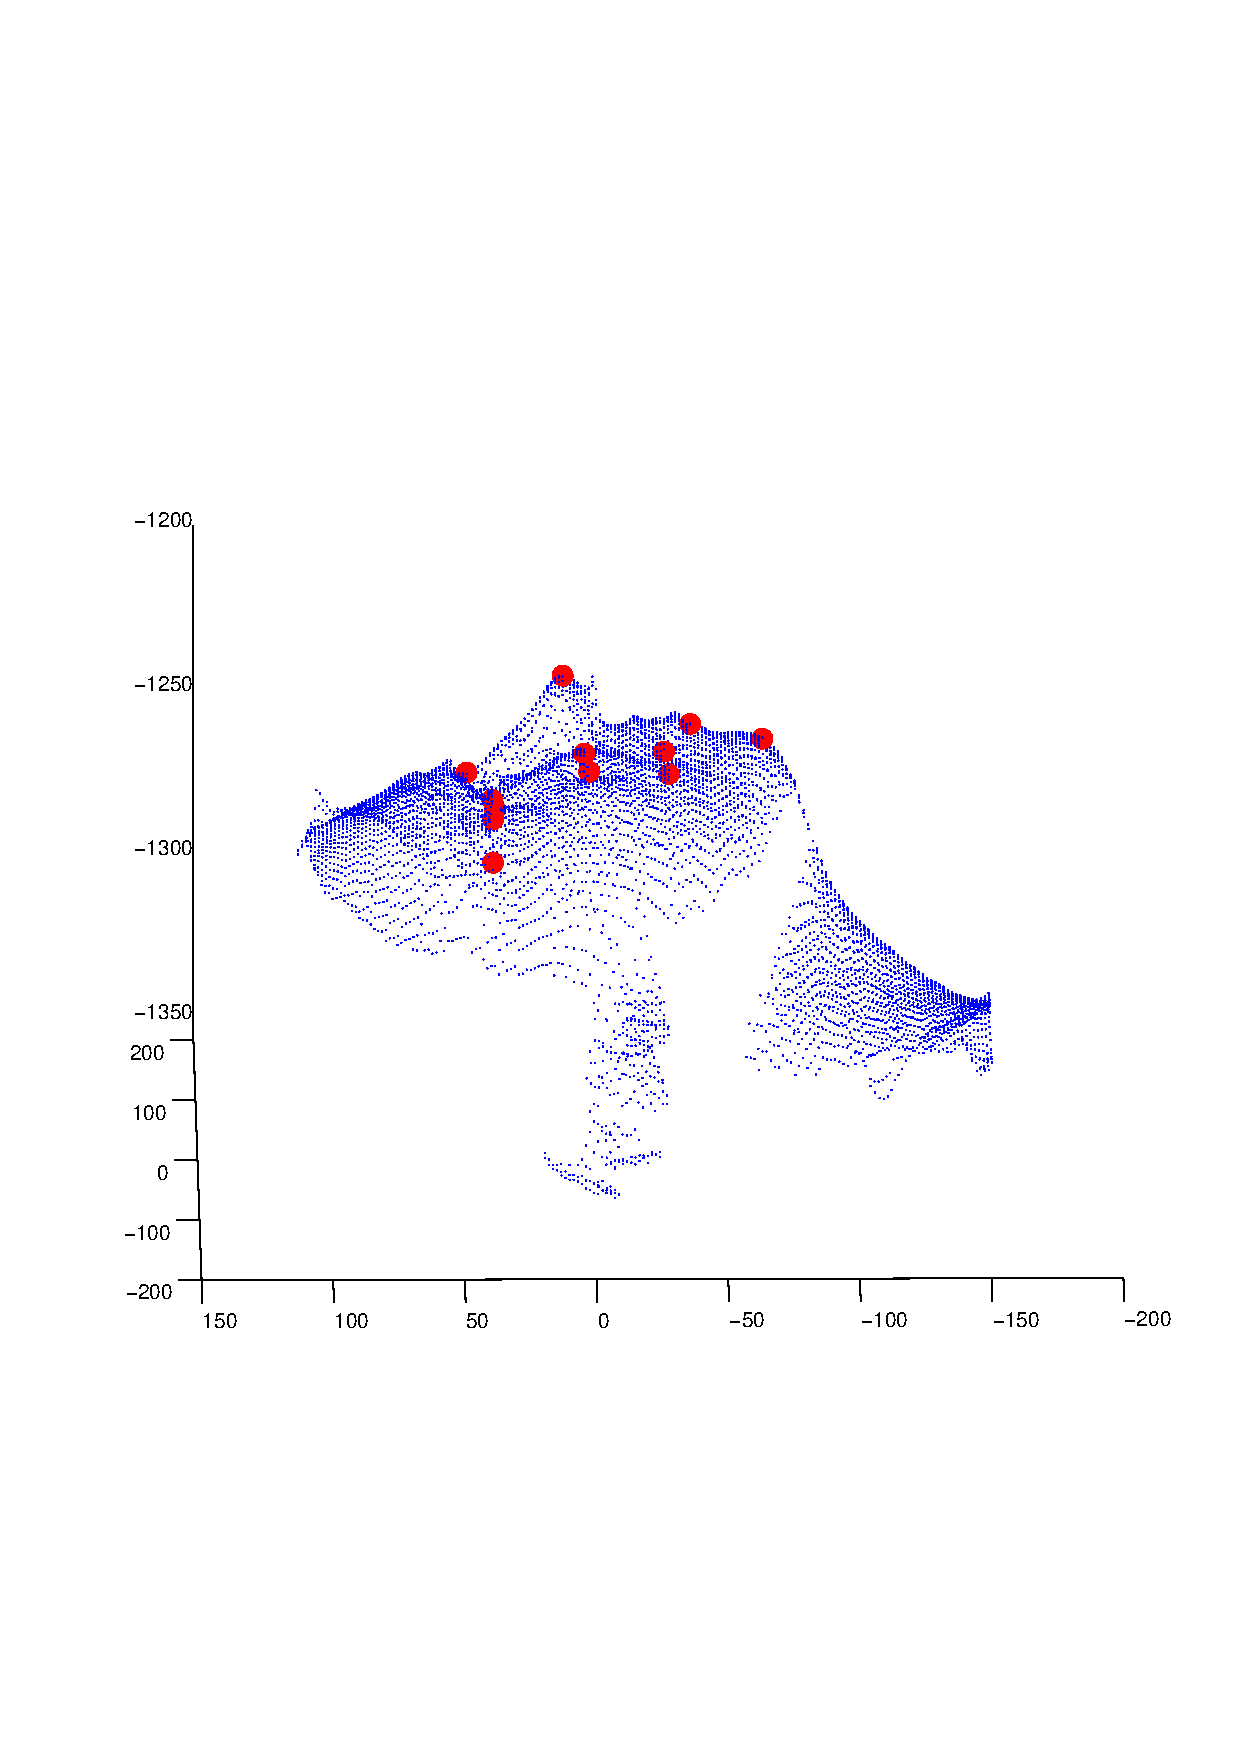
\includegraphics[width=.4\linewidth]{resources/figures/face1.png} &
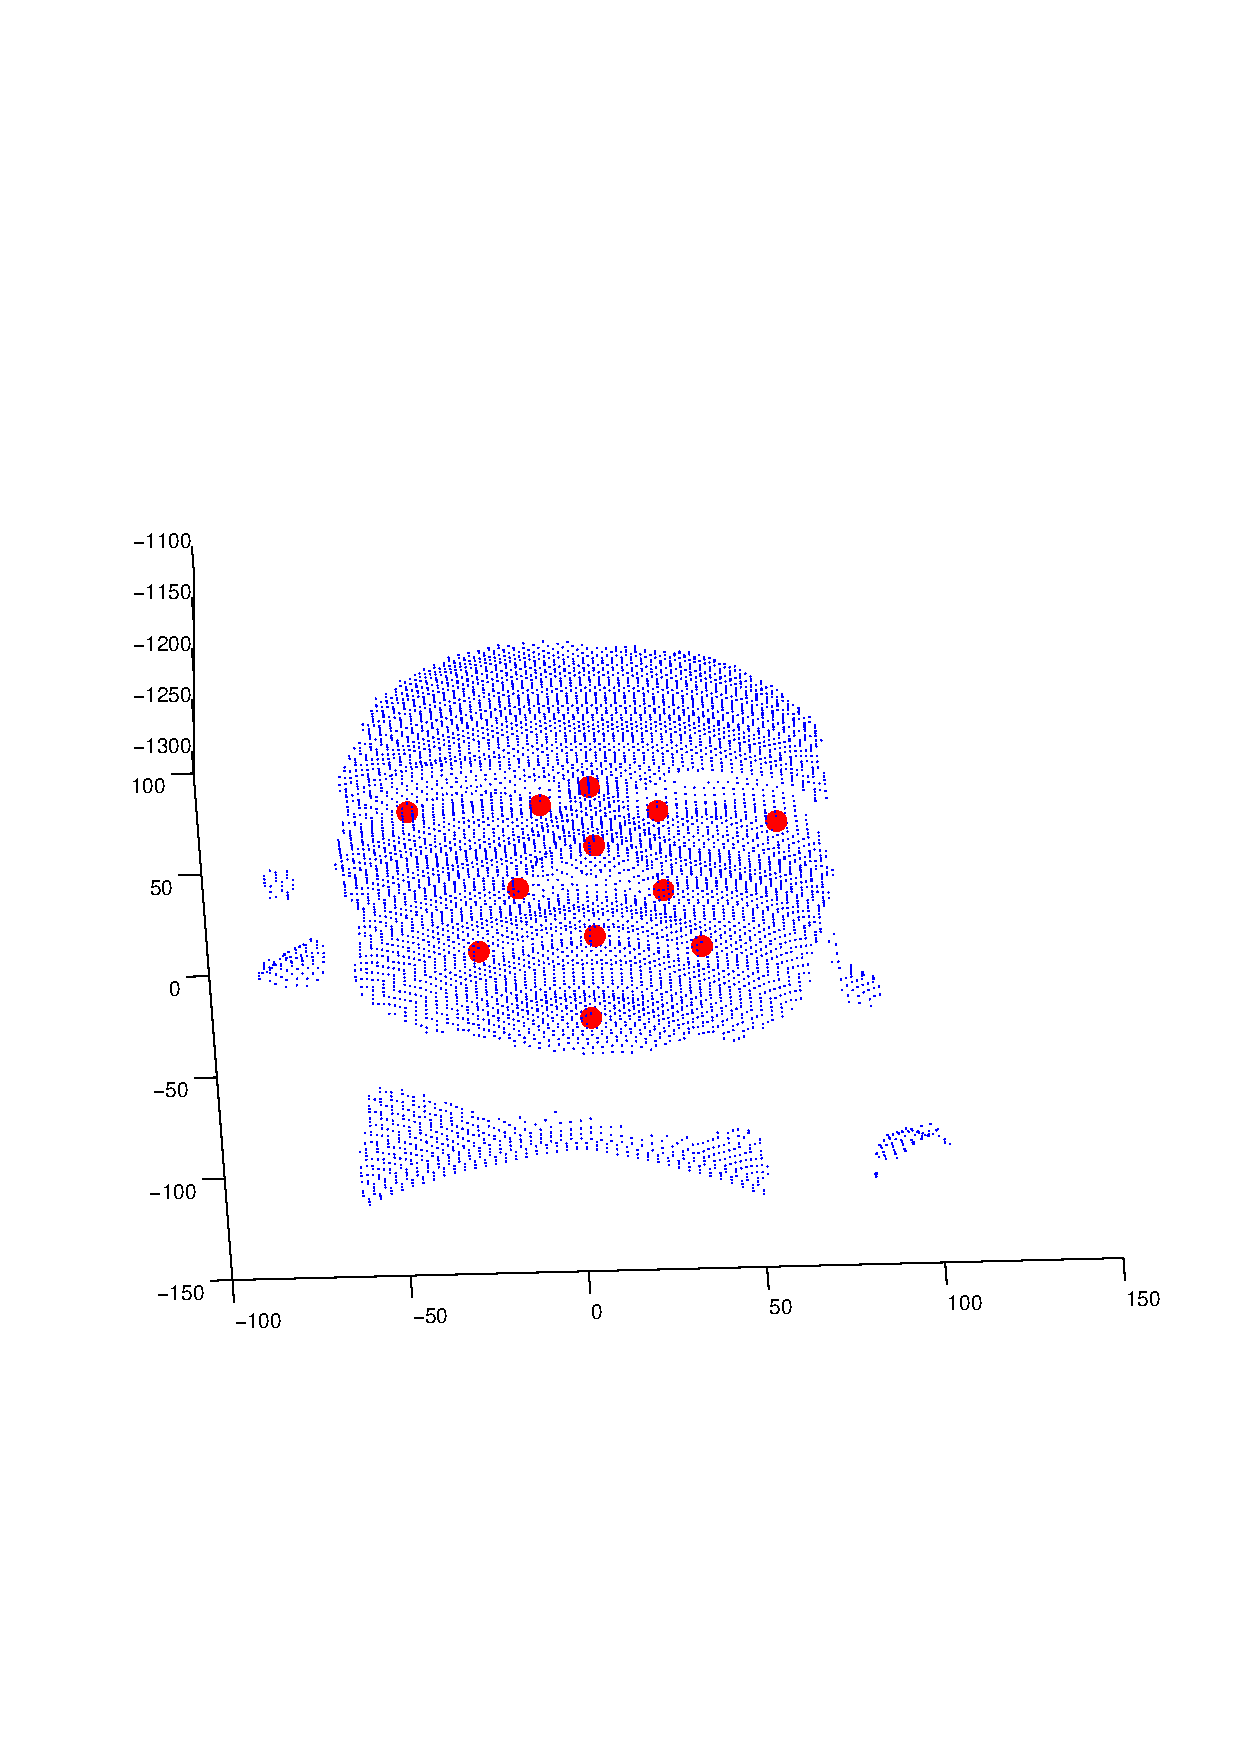
\includegraphics[width=.4\linewidth]{resources/figures/face2.png} \\
(a) & (b) \\
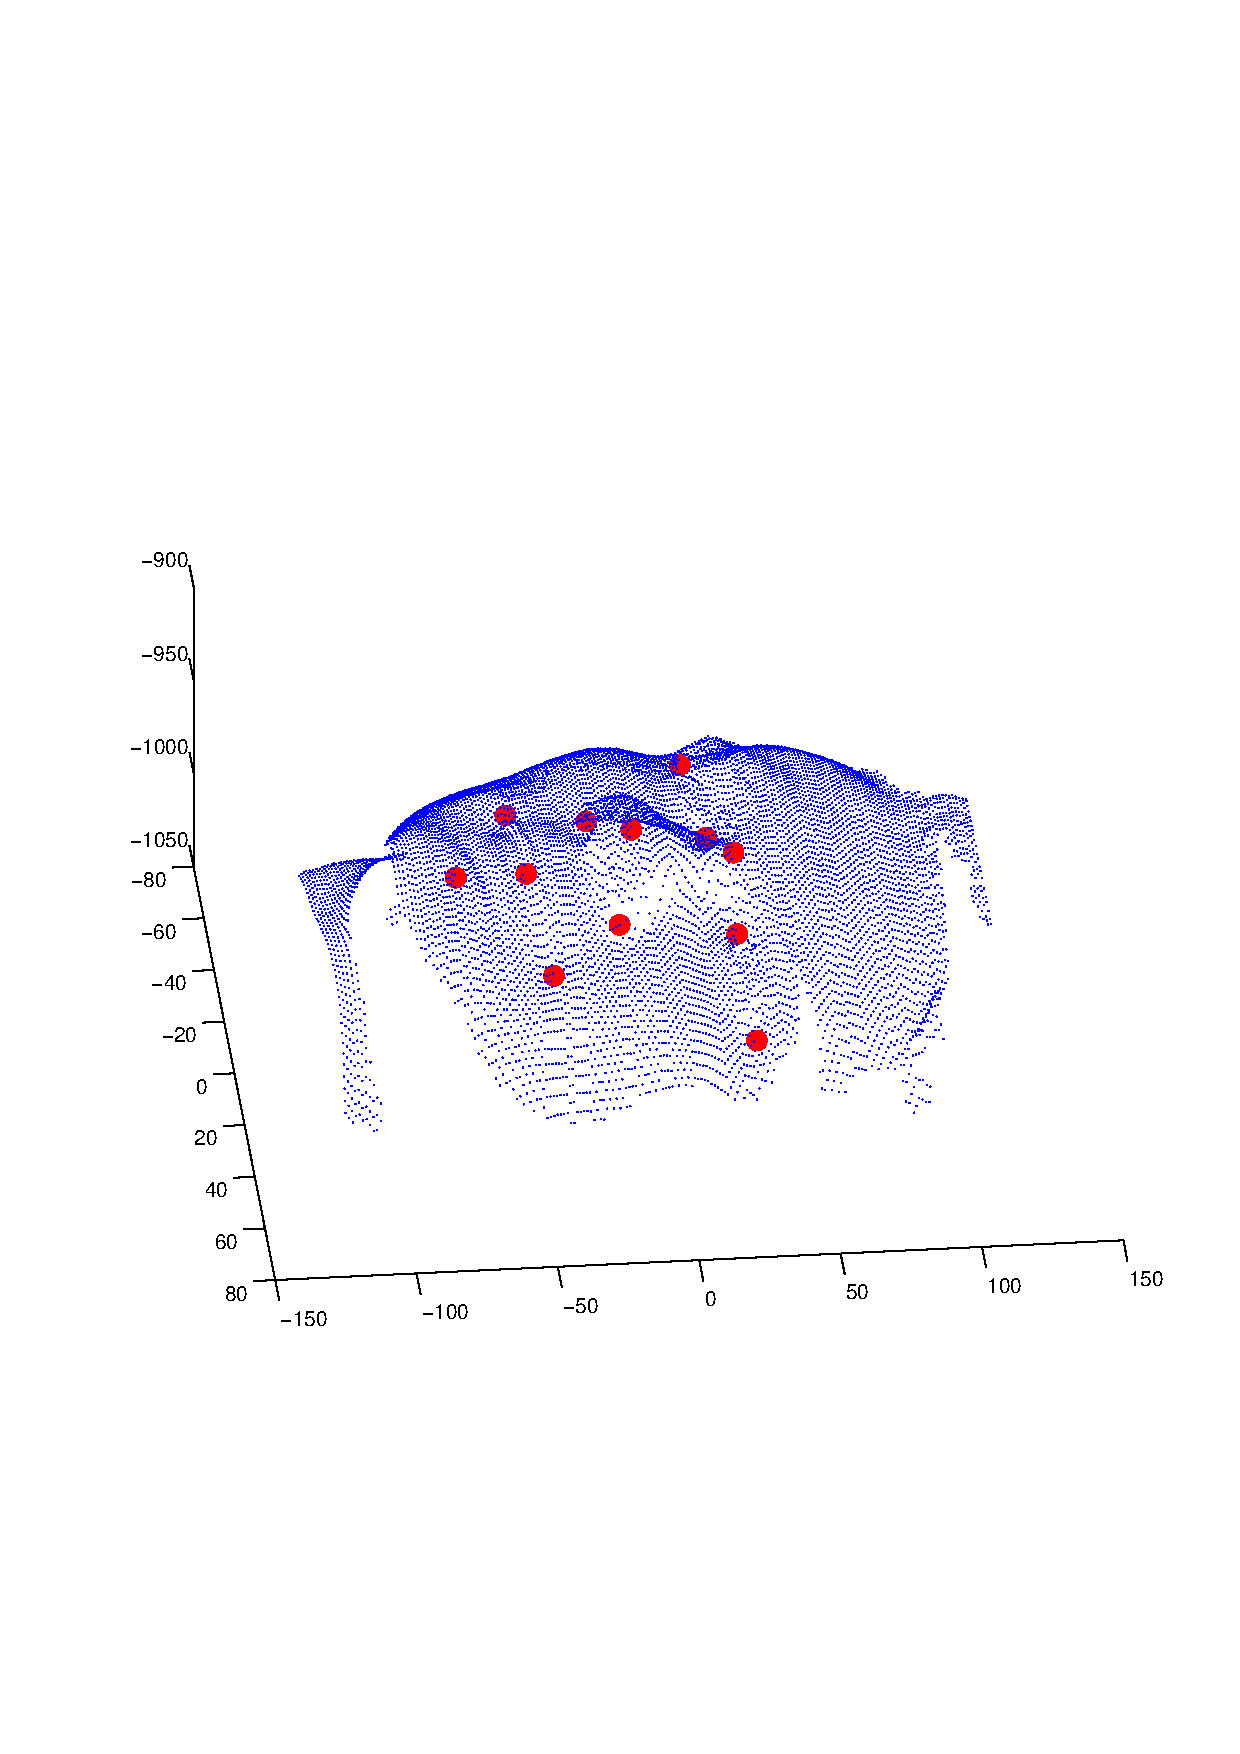
\includegraphics[width=.4\linewidth]{resources/figures/face3.png} &
\includegraphics[width=.6\linewidth]{resources/figures/fiducial_clusters.png} \\
(c) & (d)
\end{tabular}
\caption{
(a-c) show point clouds of three different faces taken from the GavaBDB \cite{moreno2004gavabdb} dataset. 
Manually clicked fiducial locations are marked with red dots.
(d) shows fiducials for 20 different faces, aligned by subtracting their respective means.  
Note the fiducials form tight clusters, meaning fiducials do not change dramatically across individuals.
This phenomenon enables robust depth estimation even for previously unseen images.
}
\label{fig:fiducial_clusters}
\end{figure}

\section{Experimental setup} \label{sec:experiments}
In this section, we show the surprising effectiveness of our method for estimating camera distance in images of previously unseen subjects.

Our experiments are run against the Texas 3D Face Recognition Database (Texas 3DFRD) \cite{gupta2010texas}; example images are shown in Figure \ref{fig:t3dfrd}.  
This database is a collection of 1149 pairs of frontal face color and depth images of 105 adult human subjects.  
Each face also has 25 manually labeled anthropometric facial fiducial points.  
Color and range images were captured simultaneously and are perfectly coregistered.  
This provides ground truth 3D locations of the fiducial locations.  

\begin{figure}[h]
\centering
\includegraphics[width=1\linewidth]{resources/figures/t3dfr.jpg}
\caption{
Example images from the Texas 3DFRD, a database of 3D scans of human faces.
These images show the 25 fiducials labeled for each face, as well as example depth maps.
}
\label{fig:t3dfrd}
\end{figure}

Our experiments consist of the following:
\begin{itemize}
\item Project fiducials for a test individual onto an image plane.
\item Use 3D fiducial locations from a set of reference individuals (not including the test individual) as exemplars.
\item For each exemplar, estimate the camera distance using the method described in Section \ref{sec:method}.
\item Repeat while simulating a dolly-zoom (or Hitchcock zoom) camera movement, in which the camera moves away as focal length is increased to keep the figure size constant.
\end{itemize}

We perform this experiment for the frontal and $3/4$ profile view of the face.  
For the frontal case, we assume all fiducials are visible to the camera.  
For the $3/4$ we assume only a subset of the fiducials are visible. 
We also assume we have a calibrated camera and all intrinsic camera parameters are known.  
Simulated camera distances range from approximately $10$cm to $3$m.
Note if we did not adjust the focal length, the distance from the camera to the face could be trivially estimated by the size of the imaged face. 
For this reason, the focal length is adjusted to keep the outermost fiducials at a near constant distance, which also keeps the imaged face silhouette at a constant size.
Results are shown in Figure \ref{fig:results}.
Our method nearly perfectly recovers camera distance.

% Figure \ref{fig:results} shows results of camera pose estimation and distance from camera to head for the frontal and $3/4$ profile views.  
% Figure \ref{fig:results} (a,c) qualitatively show the estimated camera pose.  
% The true and estimated camera distances (Figure \ref{fig:results}(b,d)) represent the distance between the camera center and tip of the nose.  
% The distance is reported in centimeters using an estimate for the average distance between outermost fiducial markers ($12$ cm).
% Note the final distance estimate closely follows the true camera distance, though the error bars get larger as the distance increases.  
% This is especially true for the $3/4$ profile view, presumably due to fewer number of visible fiducials.   

\begin{figure}[ht!]
\begin{tabular}{cc}
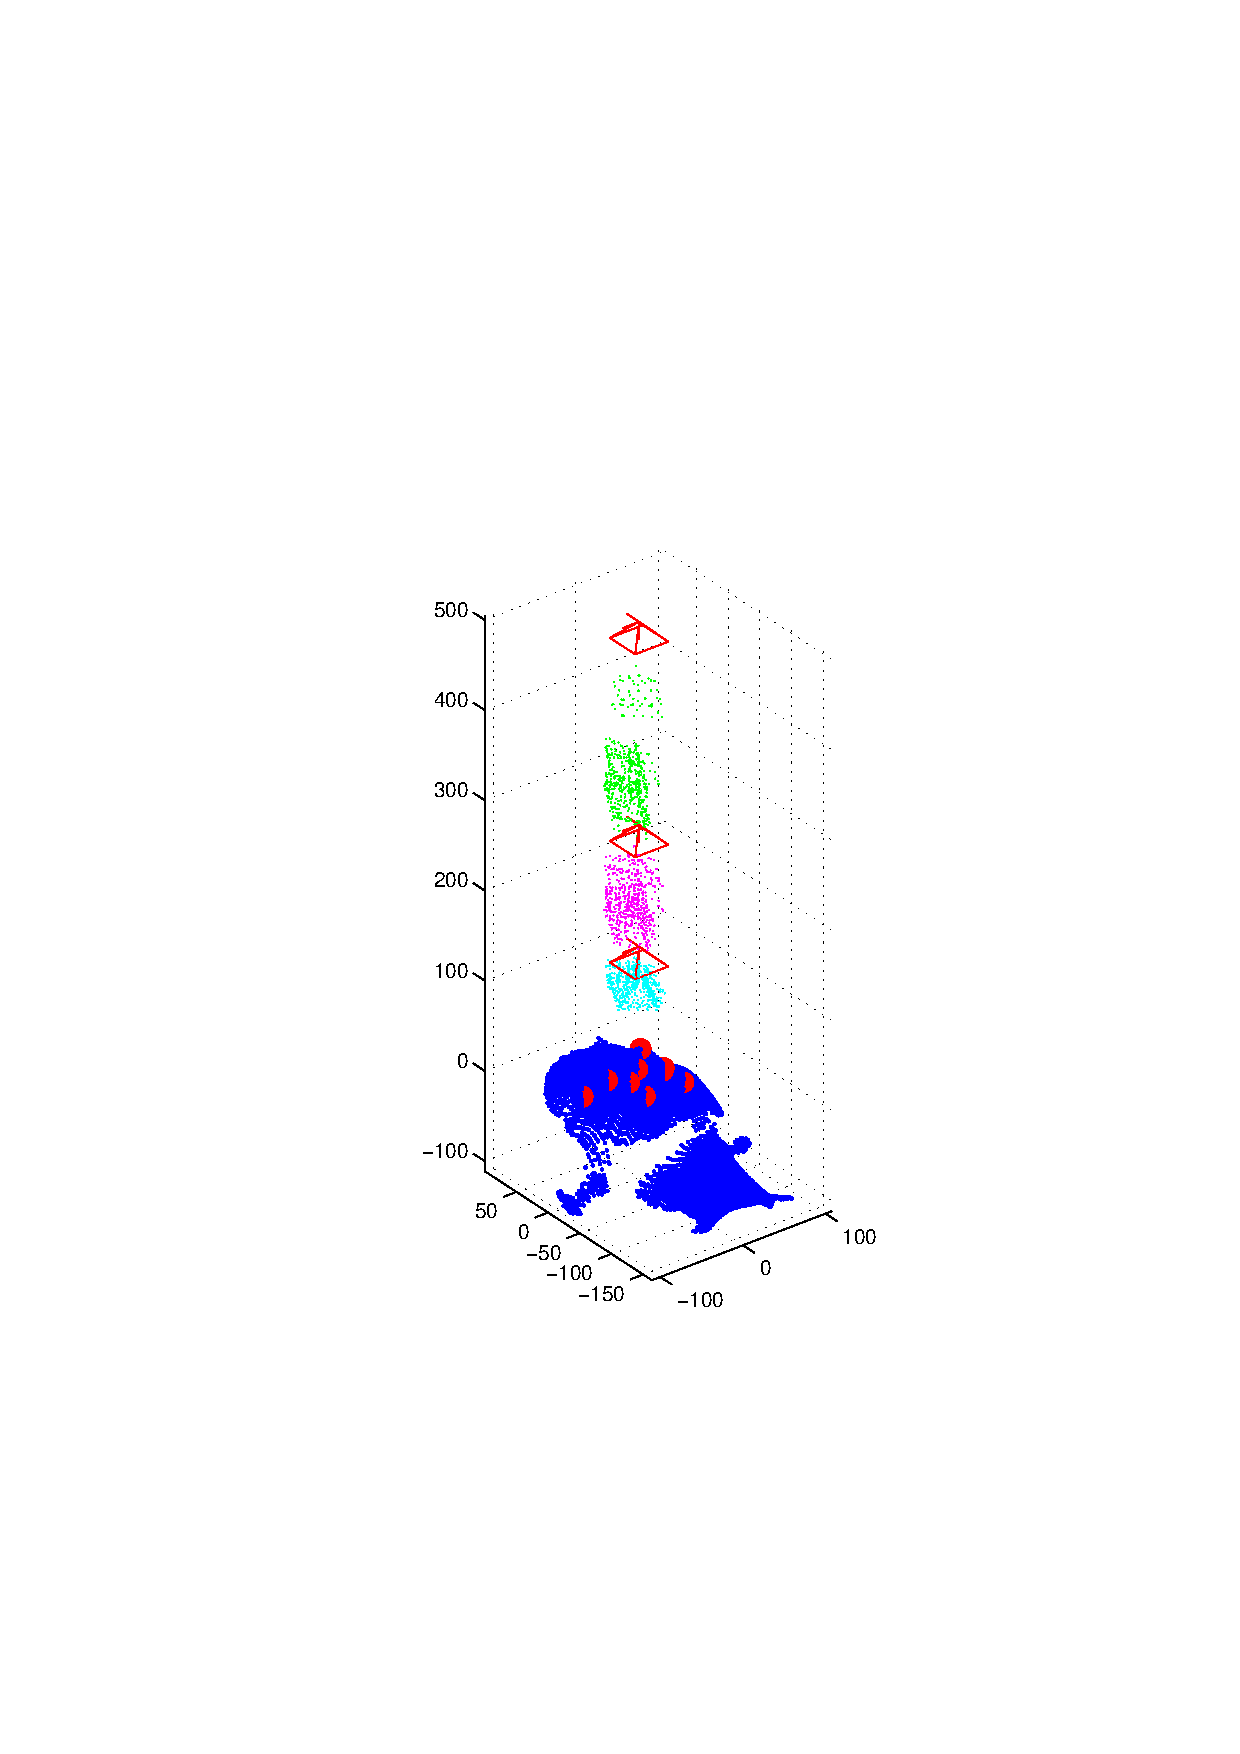
\includegraphics[width=.5\linewidth]{resources/figures/cameraloc_frontal.png} &
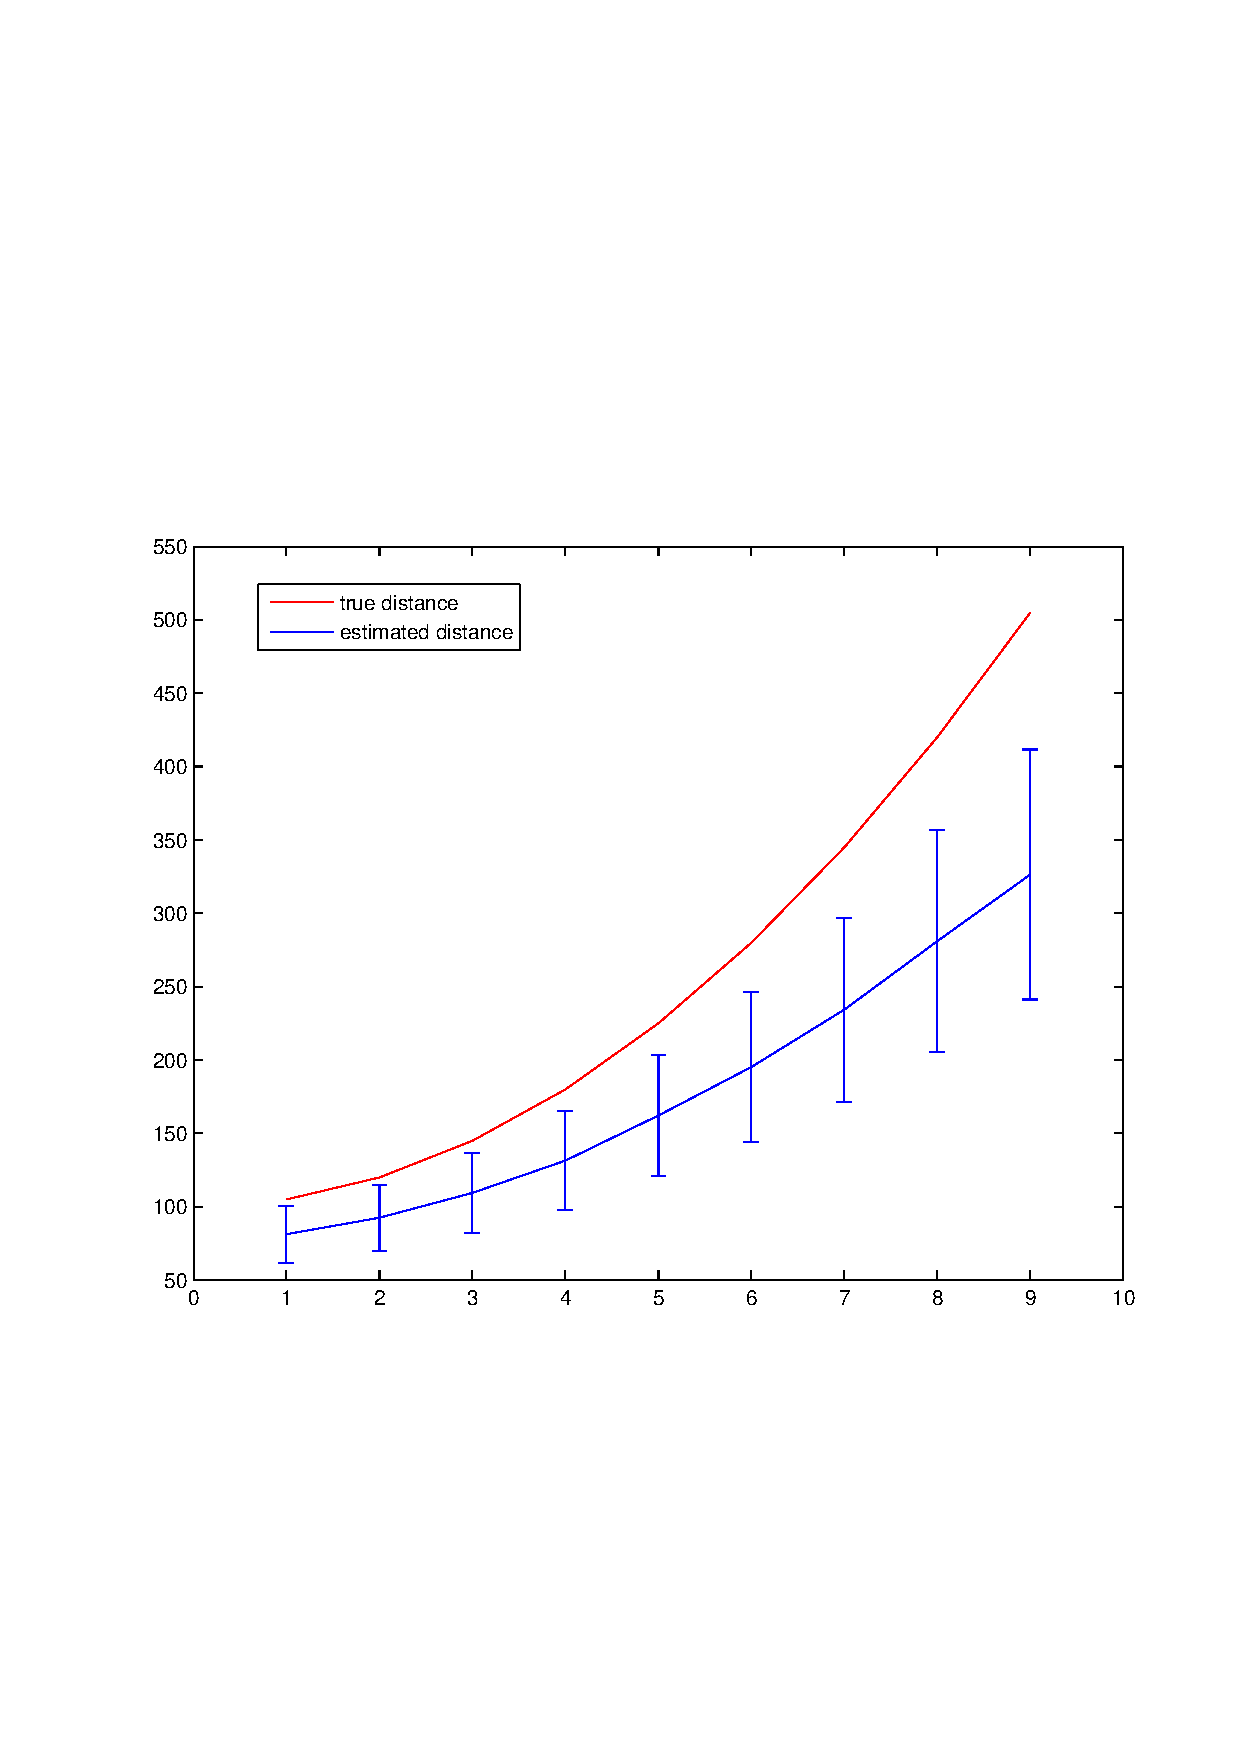
\includegraphics[width=.5\linewidth]{resources/figures/errorbar_frontal.png} \\
(a) & (b) \\
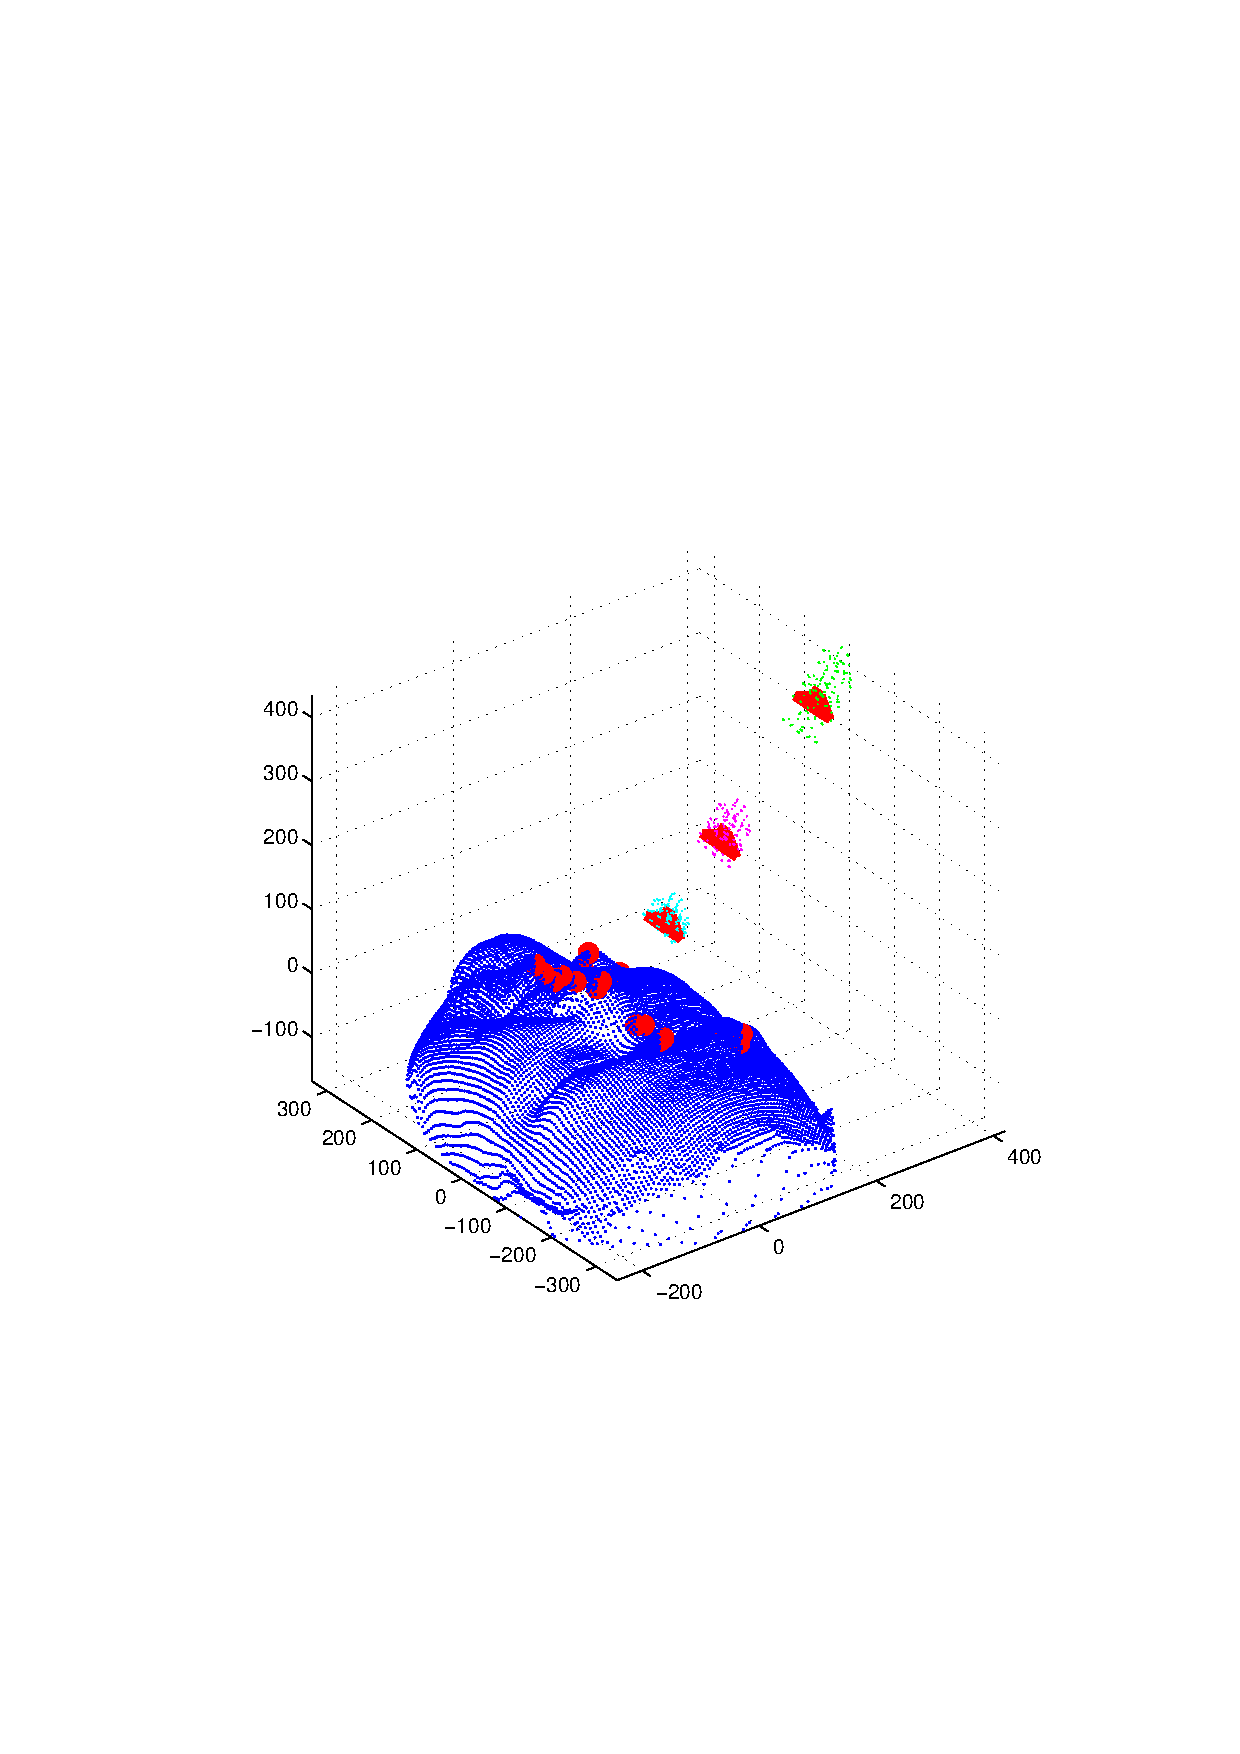
\includegraphics[width=.5\linewidth]{resources/figures/cameraloc_3q.png} &
\includegraphics[width=.5\linewidth]{resources/figures/errorbar_3q.png} \\
(c) & (d)
\end{tabular}
\caption{	
Results of camera pose and distance estimation for the frontal and $3/4$ profile views.
(a) and (c) show clusters of estimated camera poses for three distances for the frontal and $3/4$ profile views.
The clusters of poses for each of the three distances are marked using cyan, magenta, and green camera frames, with the ground truth pose marked in red.
(b) and (d) show true and estimated camera distances as a function of camera position, where distance is measured from the camera center to the tip of the nose.
We test $20$ camera positions.
The estimated distances are shown with error bars to represent the variation across exemplars.
Note the final distance estimate closely follows the true camera distance, though the error bars get larger as the distance increases.  
This is especially true for the $3/4$ profile view, presumably due to fewer number of visible fiducials.   
%  Camera pose estimation results for the frontal case.  
% True camera position is the solid red axis.  
% Estimated camera positions for near/medium/far are shown in cyan/magenta/green respectively.   
% (b) Distance estimate as an average of exemplar models.  
% We test $20$ camera positions and corresponding focal length to keep distance between outermost fiducials next to eye at a near constant. 
% (c) and (d) show equivalent results for $3/4$ profile view.
}
\label{fig:results}
\end{figure}

Figure \ref{fig:error_bar_frontal_lessfiducials} shows the same experiment where the number of fiducials is varied.  
For this experiment, we manually selected the fiducial subsets to be evenly distributed about the face.  
This figure shows the distance can be reliably estimated with as few as five fiducials.  
In the case of five fiducials, the fiducials used were outer corners of eyes and mouth, and center of top lip.
When using only four fiducials, the center of top lip was removed, resulting in 4 nearly co-planar points.
At this point, the distance estimate becomes unreliable.

\begin{figure}[h]
\centering
\includegraphics[width=1\linewidth]{resources/figures/errorbar_frontal_lessfiducials.png}
\caption{
Results of camera distance estimation for the frontal view for varying numbers of fiducials.
As in Figure \ref{fig:results}, error bars represent the variation in estimated distance across exemplars, but the actual estimate is the mean.
This shows distance can be reliably estimated with as few as five fiducials.
}
\label{fig:error_bar_frontal_lessfiducials}
\end{figure}

For qualitative analysis, we use a heuristic to select a ``best'' exemplar.  Let $p_i$ be the 2D imaged fiducial using the true camera position.  
Let $p_{ij}'$ be the imaged fiducial using the estimated camera position from the $j$-th exemplar.
We use $\argmin_j \sum_i \|p_i - p_{ij}'\|$ as a heuristic to select the best exemplar. 
See Figure \ref{fig:bestexemplar} for some illustrative examples.  
In these examples, it is interesting to see what can be recovered by simply using fiducial geometry.  
Top row shows best exemplar matches the gender of the probe image.  
Second row shows similar race in two out of three cases.  
In all cases, the general shape of the image is returned in the best matching exemplar.\afbnote{add more interesting commentary here}.

\begin{figure}[h]
\centering
\begin{tabular}{cc}
\includegraphics[width=.7\linewidth]{resources/figures/best_exemplar1.png} \\
\includegraphics[width=.7\linewidth]{resources/figures/best_exemplar3.png} \\
\includegraphics[width=.7\linewidth]{resources/figures/best_exemplar10.png} \\
\includegraphics[width=.7\linewidth]{resources/figures/best_exemplar26.png}
\end{tabular}
\caption{Best exemplar face using a heuristic of Sum of Squared error between imaged 2d fiducial points from true camera position and estimated camera position.  In each row, left column shows a probe image followed by its best matching exemplar at different camera distances. Distances (or camera positions) one, ten, and twenty correspond to physical distances of 10cm, 75cm, and 300cm, respectively. }
\label{fig:bestexemplar}
\end{figure}

\section{Conclusion and future work} \label{sec:discussion}
We have shown a method for estimating the distance from camera to a previously unseen face using correspondences of 2D imaged fiducials to 3D fiducial locations on exemplar heads.  
The distance estimate is accurate in distances ranging from 10cm to 300 cm for the frontal and $3/4$ profile views.  
Providing an estimate of this distance can be used to mitage the effects of perspective distortion in face recognition.  

In this paper, we have used a dataset consisting of facial range images with manually labelled fiducials.    
Furthermore we assume an ideal pinhole camera model and we control the pose of both head and camera.  
This simplifies the problem since we have accurate ground truth 2D and 3D fiducial locations. 
For future work, we plan to use methods for detecting fiducials such as \cite{belhumeur2011localizing}, or naturally ocurring features (e.g. SIFT features \cite{lowe}) as in \cite{ohayon2006robust}.
Replicating these results on real images is also future research direction.


\bibliographystyle{splncs}
\bibliography{library}

\end{document}
